\documentclass[11 pt]{article}
\usepackage{amsmath,amsfonts,parskip}
\usepackage[a4paper]{geometry}
\usepackage[T1]{fontenc}
\usepackage{enumerate}
\usepackage{graphicx}
\usepackage{cleveref}

\begin{document}

\begin{center}
       \large{
       \textbf{Computational Physics - PH3264} \break
	Module 2 - Integration
}
\end{center}

\textbf{Krishna Iyer V S \hfill Roll:20201017}
\hrule 
\vspace{0.3cm}
\begin{enumerate}
\item
\textbf{Euler's Method:}\\
Step Size 0.001: 7.24764\\
Step Size 00.01: 28.0671
\item
\textbf{Modified Euler's Method:}\\
Step Size 0.001: 0.07706\\
Step Size 00.01: 4.76803
\item
\textbf{Improved Euler's Method:}\\
Step Size 0.001: 0.05128\\
Step Size 00.01: 3.59668
\item
\textbf{Runge-Kutta RK-4 Method:}\\
Step Size 0.001: $3.54\cdot10^{-6}$\\
Step Size 00.01: 0.02834

\item The value of $x$ (starting with $x_0 = 0.1$ and $v_0 = 1.9$) at the end of 5000 iterations is -2.39932.
\item The value of $x$ (starting with $x_0 = 0$ and $v_0 = 1.999$) at the end of 5000 iterations is -2.34132.
\item When $v_0 > 2$, the function $x(t)$ becomes monotonously increasing. The corresponding graphs for Qn.5, Qn.6 and Qn.7 are shown in Figure \ref{fig1}.
\begin{figure}[!h]
\center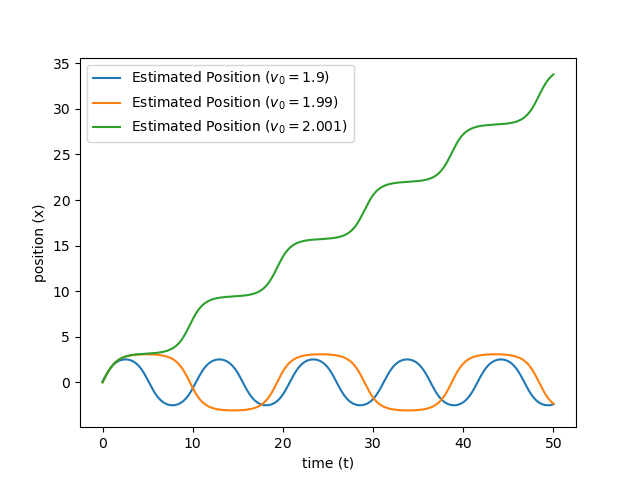
\includegraphics[width=3.7in]{"../figures/Q5-6-7.png"}
\caption{Solution for $x$ with different initial values.}
\label{fig1}
\end{figure}

\item The final $y$ value of particle 1 at $t=40$ is -0.11891. As the system is symmetric about the first and $26^{th}$. Therefore, we expect the graph for time evolution of particle 1 to be identical to that of particle 26. This has been shown in Figure \ref{fig2}.
\begin{figure}[!h]
\center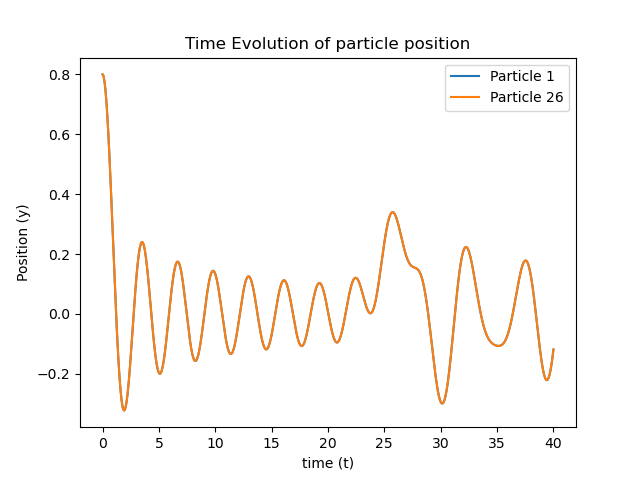
\includegraphics[width=3.7in]{"../figures/Q8_p1_26_y_vs_t.png"}
\caption{Solution for $x$ with different initial values.}
\label{fig2}
\end{figure}

\item The value of the function at $x = 0.8$ is 0.28147.
\end{enumerate}
\end{document}
